% JAA asks for IAU-format references (author initials, year, journal, volume, page), which
% mnras.bst produces. sn-jnl hard-codes its own style while loading, so we skip that one call.
\let\KernelBibStyle\bibliographystyle
\def\bibliographystyle#1{}
\documentclass[pdflatex,sn-basic]{sn-jnl}
\let\bibliographystyle\KernelBibStyle

\usepackage{graphicx}
\usepackage{amsmath,amssymb,amsfonts}
\usepackage{booktabs}
\usepackage{xcolor}
\usepackage{textcomp}

\raggedbottom

% Every result number below is a macro generated from committed result files
% (research/figures/paper_main.py and research/figures/phase4_numbers.py).
% GENERATED by research/figures/paper_main.py -- do not edit
\newcommand{\CausalBugPct}{98\%}
\newcommand{\SimGamma}{0.1}
\newcommand{\SimLengthscale}{1.2}
\newcommand{\SimNEvents}{1000}
\newcommand{\SimNModeled}{587}
\newcommand{\SimNWithheld}{413}
\newcommand{\SimHOneVerdict}{\textbf{fail}}
\newcommand{\SimHTwoVerdict}{\textbf{pass}}
\newcommand{\SimHThreeVerdict}{\textbf{pass}}
\newcommand{\SimTtiP}{23.0\,h}
\newcommand{\SimIdP}{99\%}
\newcommand{\SimTtiBzero}{$>$\,budget}
\newcommand{\SimIdBzero}{48\%}
\newcommand{\SimHolmBzero}{$<10^{-4}$}
\newcommand{\SimRbcBzero}{0.52}
\newcommand{\SimFasterBzero}{50\%}
\newcommand{\SimSlowerBzero}{48\%}
\newcommand{\SimTtiBone}{12.05\,d}
\newcommand{\SimIdBone}{61\%}
\newcommand{\SimHolmBone}{$<10^{-4}$}
\newcommand{\SimRbcBone}{0.63}
\newcommand{\SimFasterBone}{62\%}
\newcommand{\SimSlowerBone}{27\%}
\newcommand{\SimTtiBtwo}{13.8\,h}
\newcommand{\SimIdBtwo}{72\%}
\newcommand{\SimHolmBtwo}{0.00019}
\newcommand{\SimRbcBtwo}{0.19}
\newcommand{\SimFasterBtwo}{30\%}
\newcommand{\SimSlowerBtwo}{49\%}
\newcommand{\SimTtiBthree}{1.59\,d}
\newcommand{\SimIdBthree}{99\%}
\newcommand{\SimHolmBthree}{$<10^{-4}$}
\newcommand{\SimRbcBthree}{0.33}
\newcommand{\SimFasterBthree}{48\%}
\newcommand{\SimSlowerBthree}{25\%}
\newcommand{\SimObsP}{4.2}
\newcommand{\SimObsBthree}{2.9}
\newcommand{\SimHtwoFast}{0.414}
\newcommand{\SimHtwoSlow}{0.152}
\newcommand{\SimHtwoEst}{0.261}
\newcommand{\SimHtwoCI}{[0.153, 0.368]}
\newcommand{\SimHtwoFastCI}{[0.314, 0.514]}
\newcommand{\SimHtwoSlowCI}{[0.113, 0.195]}
\newcommand{\SimTprP}{96\%}
\newcommand{\SimTprBthree}{21\%}
\newcommand{\SimHthreeEst}{76}
\newcommand{\SimHthreeCI}{[66, 84]}
\newcommand{\SimAucP}{0.993}
\newcommand{\SimAucBthree}{0.666}
\newcommand{\SimAucBtwo}{0.696}
\newcommand{\SimAucPown}{0.714}
\newcommand{\SimTprPown}{21\%}
\newcommand{\SimCwWhBthree}{97\%}
\newcommand{\SimCwWhP}{6\%}
\newcommand{\SimAccModP}{100\%}
\newcommand{\SimAccModBthree}{100\%}
\newcommand{\SimFaP}{0\%}
\newcommand{\SimFaPModelError}{13\%}
\newcommand{\SimAccModPModelError}{87\%}
\newcommand{\SimAucPModelError}{0.891}
\newcommand{\SimAucBthreeModelError}{0.706}
\newcommand{\SimAucPCrowding}{0.975}
\newcommand{\SimObsAllP}{4.2}
\newcommand{\SimAccModPAll}{100\%}
\newcommand{\SimCwWhPAll}{6\%}
\newcommand{\SimFlagP}{89\%}
\newcommand{\SimAucAblP}{0.993}
\newcommand{\SimObsAllNoDecay}{3.6}
\newcommand{\SimAccModNoDecayAll}{99\%}
\newcommand{\SimCwWhNoDecayAll}{31\%}
\newcommand{\SimFlagNoDecay}{65\%}
\newcommand{\SimAucAblNoDecay}{0.936}
\newcommand{\SimObsAllNoAdeq}{4.3}
\newcommand{\SimAccModNoAdeqAll}{100\%}
\newcommand{\SimCwWhNoAdeqAll}{6\%}
\newcommand{\SimFlagNoAdeq}{89\%}
\newcommand{\SimAucAblNoAdeq}{0.992}
\newcommand{\SimObsAllBthree}{2.8}
\newcommand{\SimAccModBthreeAll}{100\%}
\newcommand{\SimCwWhBthreeAll}{97\%}
\newcommand{\SimObsAllBtwo}{4.9}
\newcommand{\SimAccModBtwoAll}{88\%}
\newcommand{\SimCwWhBtwoAll}{69\%}
\newcommand{\SimObsAllBone}{3.2}
\newcommand{\SimAccModBoneAll}{80\%}
\newcommand{\SimCwWhBoneAll}{75\%}
\newcommand{\SimObsAllBzero}{5.0}
\newcommand{\SimAccModBzeroAll}{79\%}
\newcommand{\SimCwWhBzeroAll}{1\%}
\newcommand{\SimDeltaKilonova}{1.59}
\newcommand{\SimDeltaShock}{0.32}
\newcommand{\SimDeltaFlare}{-0.56}
\newcommand{\SimDeltaGrb}{0.15}
\newcommand{\SimHtwoModelErrorEst}{-0.098}
\newcommand{\SimHtwoModelErrorCI}{[-0.171, -0.024]}
\newcommand{\SimHtwoCrowdingEst}{0.232}
\newcommand{\SimHthreeModelErrorEst}{17}
\newcommand{\SimHthreeModelErrorCI}{[8, 31]}
\newcommand{\SimAccModBthreeModelError}{99\%}
\newcommand{\SimHOneCrowding}{fail}
\newcommand{\SimHTwoCrowding}{pass}
\newcommand{\SimHThreeCrowding}{pass}
\newcommand{\SimHOneModelError}{fail}
\newcommand{\SimHTwoModelError}{fail}
\newcommand{\SimHThreeModelError}{pass}
\newcommand{\RealCHOneVerdict}{\textbf{pass}}
\newcommand{\RealCHTwoVerdict}{\textbf{pass}}
\newcommand{\RealCHThreeVerdict}{\textbf{pass}}
\newcommand{\RealCHFourVerdict}{\textbf{pass}}
\newcommand{\RealCHFiveVerdict}{\textbf{fail}}
\newcommand{\RealRHOneVerdict}{\textbf{pass}}
\newcommand{\RealRHTwoVerdict}{\textbf{pass}}
\newcommand{\RealRHThreeVerdict}{\textbf{fail}}
\newcommand{\RealRHFourVerdict}{\textbf{pass}}
\newcommand{\RealRHFiveVerdict}{\textbf{fail}}
\newcommand{\RealNEvents}{364}
\newcommand{\RealNWithheld}{88}
\newcommand{\RealNModeled}{276}
\newcommand{\RealCAuc}{0.79--0.81}
\newcommand{\RealCCwWhBthree}{50--56\%}
\newcommand{\RealCAccModBthree}{58--62\%}
\newcommand{\RealCCwWhP}{7--14\%}
\newcommand{\RealCAccModP}{59--63\%}
\newcommand{\RealCCwWhBone}{40--45\%}
\newcommand{\RealCAccModBone}{54--56\%}
\newcommand{\RealCFlagP}{39--47\%}
\newcommand{\RealCFaP}{8\%}
\newcommand{\RealRAuc}{0.77--0.80}
\newcommand{\RealRCwWhBthree}{78--80\%}
\newcommand{\RealRAccModBthree}{59--62\%}
\newcommand{\RealRCwWhP}{12--19\%}
\newcommand{\RealRAccModP}{53--54\%}
\newcommand{\RealRCwWhBone}{48--49\%}
\newcommand{\RealRAccModBone}{51--55\%}
\newcommand{\RealRFlagP}{64--73\%}
\newcommand{\RealRFaP}{24--25\%}
\newcommand{\RealCObsP}{2.3}
\newcommand{\RealCObsBthree}{2.6}
\newcommand{\RealCObsBzero}{5.0}
\newcommand{\RealRObsP}{5.0}
\newcommand{\RealRObsBthree}{5.0}
\newcommand{\RealRObsBzero}{5.0}
\newcommand{\ConfAlpha}{0.1}
\newcommand{\ConfAlphaPct}{10\%}
\newcommand{\ConfLambda}{0.25}
\newcommand{\ConfNFresh}{489}
\newcommand{\ConfNCal}{456}
\newcommand{\ConfHCOneVerdict}{\textbf{pass}}
\newcommand{\ConfHCTwoVerdict}{\textbf{pass}}
\newcommand{\ConfHCThreeVerdict}{\textbf{pass}}
\newcommand{\ConfHCFourVerdict}{\textbf{pass}}
\newcommand{\ConfHCFiveVerdict}{\textbf{pass}}
\newcommand{\ConfHCSixVerdict}{\textbf{fail}}
\newcommand{\ConfFa}{3--6\%}
\newcommand{\ConfAccGain}{6--8~points}
\newcommand{\ConfFlag}{42--55\%}
\newcommand{\ConfAucGain}{+0.012--+0.039}
\newcommand{\ConfAccFreshCL}{66--69\%}
\newcommand{\ConfAccFreshP}{61--66\%}
\newcommand{\ConfAccFreshBthree}{60\%}
\newcommand{\ConfAccFreshBthreeConf}{57--58\%}
\newcommand{\ConfRawFaFreshP}{7--9\%}
\newcommand{\ConfCwUnkCL}{26--32\%}
\newcommand{\ConfCwUnkP}{7--14\%}
\newcommand{\ConfCwUnkBthree}{50--56\%}
\newcommand{\ConfFlagBthreeConf}{41--52\%}
\newcommand{\ConfObsP}{2.3--2.4}
\newcommand{\ConfObsL}{3.1--3.2}

% GENERATED by research/figures/phase4_numbers.py -- do not edit
\newcommand{\FleetNEpisodes}{250}
\newcommand{\FleetNEvents}{1000}
\newcommand{\FleetNModeled}{592}
\newcommand{\FleetNUnknown}{408}
\newcommand{\FleetReserveA}{10}
\newcommand{\FleetReserveG}{3}
\newcommand{\FleetReserveK}{10}
\newcommand{\FleetReserveO}{1}
\newcommand{\FleetHFourOneVerdict}{\textbf{pass}}
\newcommand{\FleetHFourOneEst}{+10.5}
\newcommand{\FleetHFourOneCI}{[+6.3, +14.5]}
\newcommand{\FleetHFourTwoVerdict}{\textbf{fail}}
\newcommand{\FleetHFourTwoEst}{-1.5}
\newcommand{\FleetHFourTwoCI}{[-5.4, +2.3]}
\newcommand{\FleetHFourThreeVerdict}{\textbf{pass}}
\newcommand{\FleetHFourThreeEst}{+12.0}
\newcommand{\FleetHFourThreeCI}{[+8.2, +15.8]}
\newcommand{\FleetHFourFourVerdict}{\textbf{pass}}
\newcommand{\FleetHFourFourEst}{+0.5}
\newcommand{\FleetHFourFourCI}{[-1.8, +2.8]}
\newcommand{\FleetHEOneVerdict}{\textbf{pass}}
\newcommand{\FleetHETwoVerdict}{\textbf{pass}}
\newcommand{\FleetHEOneMaxK}{1}
\newcommand{\FleetHEOneN}{592}
\newcommand{\FleetHEOneMaxUpper}{0.008}
\newcommand{\FleetHETwoK}{0}
\newcommand{\FleetHETwoN}{4736}
\newcommand{\FleetAccO}{87\%}
\newcommand{\FleetObsO}{5.1}
\newcommand{\FleetLsO}{-0.80}
\newcommand{\FleetAucO}{0.93}
\newcommand{\FleetCwUO}{8\%}
\newcommand{\FleetFlagO}{48\%}
\newcommand{\FleetEDetO}{26\%}
\newcommand{\FleetStaleO}{0\%}
\newcommand{\FleetDupO}{2.3}
\newcommand{\FleetAccG}{76\%}
\newcommand{\FleetObsG}{5.4}
\newcommand{\FleetLsG}{-0.99}
\newcommand{\FleetAucG}{0.88}
\newcommand{\FleetCwUG}{4\%}
\newcommand{\FleetFlagG}{39\%}
\newcommand{\FleetEDetG}{16\%}
\newcommand{\FleetStaleG}{88\%}
\newcommand{\FleetDupG}{2.0}
\newcommand{\FleetAccA}{75\%}
\newcommand{\FleetObsA}{3.7}
\newcommand{\FleetLsA}{-0.88}
\newcommand{\FleetAucA}{0.90}
\newcommand{\FleetCwUA}{0\%}
\newcommand{\FleetFlagA}{45\%}
\newcommand{\FleetEDetA}{21\%}
\newcommand{\FleetStaleA}{29\%}
\newcommand{\FleetDupA}{1.3}
\newcommand{\FleetAccK}{74\%}
\newcommand{\FleetObsK}{3.8}
\newcommand{\FleetLsK}{-0.91}
\newcommand{\FleetAucK}{0.89}
\newcommand{\FleetCwUK}{0\%}
\newcommand{\FleetFlagK}{42\%}
\newcommand{\FleetEDetK}{19\%}
\newcommand{\FleetStaleK}{29\%}
\newcommand{\FleetDupK}{1.4}
\newcommand{\FleetAccAOne}{72\%}
\newcommand{\FleetObsAOne}{3.8}
\newcommand{\FleetLsAOne}{-0.95}
\newcommand{\FleetAucAOne}{0.88}
\newcommand{\FleetCwUAOne}{1\%}
\newcommand{\FleetFlagAOne}{39\%}
\newcommand{\FleetEDetAOne}{14\%}
\newcommand{\FleetStaleAOne}{45\%}
\newcommand{\FleetDupAOne}{1.2}
\newcommand{\FleetLinkUpOne}{1\%}
\newcommand{\FleetLinkUpFive}{12\%}
\newcommand{\FleetMEFalseUnknownO}{14\%}
\newcommand{\FleetMEFalseUnknownG}{5\%}
\newcommand{\FleetExAminusGEst}{+2.4}
\newcommand{\FleetExAminusGCI}{[-1.0, +5.6]}
\newcommand{\FleetExOminusGEst}{+5.1}
\newcommand{\FleetExOminusGCI}{[+1.0, +9.1]}
\newcommand{\FleetExOminusAEst}{+2.7}
\newcommand{\FleetExOminusACI}{[-0.7, +6.2]}
\newcommand{\FleetExAminusKEst}{-0.5}
\newcommand{\FleetExAminusKCI}{[-3.0, +1.9]}
\newcommand{\FleetExAccO}{81\%}
\newcommand{\FleetBOneVerdict}{\textbf{pass}}
\newcommand{\FleetBOneEst}{+5.3}
\newcommand{\FleetBOneCI}{[+2.9, +7.6]}
\newcommand{\FleetBOneMag}{5.3}
\newcommand{\FleetBTwoVerdict}{\textbf{pass}}
\newcommand{\FleetBTwoEst}{-1.3}
\newcommand{\FleetBTwoCI}{[-3.0, +0.5]}
\newcommand{\FleetBTwoMag}{1.3}
\newcommand{\FleetBThreeVerdict}{\textbf{pass}}
\newcommand{\FleetBThreeEst}{+7.9}
\newcommand{\FleetBThreeCI}{[+5.9, +9.8]}
\newcommand{\FleetBThreeMag}{7.9}
\newcommand{\FleetBFourVerdict}{\textbf{pass}}
\newcommand{\FleetBFourEst}{+9.4}
\newcommand{\FleetBFourCI}{[+6.9, +12.0]}
\newcommand{\FleetBFourMag}{9.4}
\newcommand{\FleetHFourOneMag}{10.5}
\newcommand{\FleetBFiveVerdict}{\textbf{pass}}
\newcommand{\FleetBFiveEst}{+0.27}
\newcommand{\FleetBFiveCI}{[+0.23, +0.31]}
\newcommand{\FleetBDenseAGEst}{+1.8}
\newcommand{\FleetBDenseAGCI}{[-0.8, +4.4]}
\newcommand{\FleetBNEvents}{2000}
\newcommand{\FleetDenseLinkUpOne}{9\%}
\newcommand{\FleetDenseLinkUpFive}{38\%}
\newcommand{\FleetBAccOSparse}{80\%}
\newcommand{\FleetBAccODense}{70\%}
\newcommand{\ECalFa}{3.9--5.0\%}
\newcommand{\ECalN}{456}
\newcommand{\EHROneVerdict}{\textbf{pass}}
\newcommand{\EHRTwoVerdict}{\textbf{pass}}
\newcommand{\EFreshN}{489}
\newcommand{\EWithheldN}{88}
\newcommand{\EFreshFa}{3.3--4.3\%}
\newcommand{\EFreshFaUpper}{6.1\%}
\newcommand{\EDet}{26--31\%}
\newcommand{\EDetLower}{19\%}
\newcommand{\EDetBthree}{36--41\%}
\newcommand{\EFreshFaBthree}{5.1--6.1\%}
\newcommand{\EDetL}{40--50\%}


\begin{document}

\title[None of the Above, Across a Fleet]{Knowing What You Do Not Know: Open-World Follow-Up Planning for Fading Transients, from One Spacecraft to a Fleet}

\author*[1]{\fnm{Joyce} \sur{Malik}}\email{joycemalik14@gmail.com (ORCID: \href{https://orcid.org/0009-0001-8293-8064}{0009-0001-8293-8064})}
\author[1]{\fnm{Anup} \sur{H}}
\author[1]{\fnm{Moghitha} \sur{B}}
\author[1]{\fnm{Swathi} \sur{Satish}}

\affil*[1]{\orgdiv{Department of Computer Science and Engineering}, \orgname{Dr.\ Ambedkar Institute of Technology}, \orgaddress{\street{Outer Ring Road, Mallathahalli}, \city{Bengaluru}, \postcode{560056}, \state{Karnataka}, \country{India}}}

\abstract{Sky surveys find more short-lived explosions than any telescope can follow, so future spacecraft will have to decide what to measure next. Today's planners choose the measurement that best separates the object types they already know. But when something new appears, they have no way to say so, and every extra measurement makes them more sure of a wrong answer. We give the planner one more option, ``none of the above'', and let it measure only forward in time, as a real spacecraft must. In simulation it recognised \SimTprP\ of never-seen object types at a 5\% false-alarm rate, against \SimTprBthree\ for the usual approach. On \RealNEvents\ real transients from the Zwicky Transient Facility, it was confidently wrong about \RealCCwWhP\ of the unfamiliar objects, against \RealCCwWhBthree. We then give the word ``unknown'' a false-alarm guarantee that holds at every step, and spread the planner over satellites that can only talk when they see each other. Sharing observations helped, but where the satellites sit mattered more, and a well-connected fleet in one orbital plane was \FleetBFourMag\ percentage points less accurate than a spread one. All hypotheses were registered before testing, and we report the failures too.}

\keywords{transient follow-up, open-set recognition, Bayesian experimental design, anytime-valid inference, distributed spacecraft autonomy, preregistration}

\maketitle

\section{Introduction}\label{sec:intro}

Wide-field surveys now find far more transients than any follow-up programme can observe \citep{Bellm2019,Ivezic2019}. Many of these events fade within hours, so the measurements that would separate one explanation from another are only available for a short time. Choosing the next measurement is therefore a planning problem. The standard way to plan it is to pick the measurement with the highest expected information gain (EIG) about the event's class \citep{Lindley1956,Chaloner1995}.

EIG is good at telling known classes apart. It cannot tell us when an event belongs to none of them. A posterior over $K$ known classes always sums to one, so when a genuinely new object comes in, every new measurement pushes the planner further towards whichever known class fits least badly. The planner becomes more confident exactly when it should become less confident. The problem sits in the hypothesis space itself, so tuning will not fix it. A threshold on closed-world uncertainty fails for the same reason, since a confident wrong answer has low entropy.

We start from this observation and ask four questions. For each one, the hypotheses were committed before the test data were run.
\begin{enumerate}
\item Does adding an explicit unmodelled hypothesis $h_0$ to the planner stop it from confidently misclassifying unknown events, and what does that cost on known ones? We test this in simulation (Sect.~\ref{sec:sim}) and on real ZTF events (Sect.~\ref{sec:real}).
\item Can the ``unknown'' decision come with a guaranteed false-alarm rate? We try a conformal threshold (Sect.~\ref{sec:conf}) and anytime-valid e-values (Sect.~\ref{sec:fleet}).
\item How does respecting the order of time change these conclusions? (Sect.~\ref{sec:disc})
\item When the planner runs on a fleet whose spacecraft can only talk while in line of sight, how much does communication help, and does coordinating plans add anything beyond sharing data? (Sect.~\ref{sec:fleet})
\end{enumerate}

Our main findings and contributions are:
\begin{itemize}
\item In simulation and on real events, the open-world posterior is the part that matters. An extra utility term aimed at testing $h_0$ adds nothing.
\item We give two ways to attach a guarantee to ``unknown''. The first is a split-conformal threshold. The second, new here, is a universal-inference e-process. It is valid at every step, needs no calibration data, and can be combined across spacecraft by simple averaging.
\item We measure how a causal time order changes the conclusions of follow-up studies.
\item We build a decentralised fleet that shares observations as conflict-free replicated data types (CRDTs), and we measure what communication and coordination are worth under real link geometry.
\end{itemize}

\section{Related work and the gap}\label{sec:related}

\paragraph{Anomaly and out-of-taxonomy detection.} Broker-level systems rank alerts by how unusual they look. They use deep embeddings with isolation forests \citep{Villar2021}, real-time similarity search \citep{Aleo2024}, autoencoders on the ZTF stream \citep{Iskandarli2026}, active anomaly detection in Fink \citep{Pruzhinskaya2026} and classifier-based multi-class anomaly scores \citep{Gupta2024}. FLARE runs out-of-taxonomy detection in production \citep{Sasli2026FLARE} and reports that blind detection recovers few out-of-taxonomy objects at a 1\% false-alarm rate. ASTRANet adds conformal calibration to spectroscopic classification \citep{Sasli2026ASTRANet}. All of these work on data that already exist, so none of them decides which measurement to take next to make the unknown recognisable.

\paragraph{Information-driven follow-up.} Information-theoretic and active-learning methods choose which objects deserve a spectrum \citep{Astudillo2020,Kennamer2020,Moller2025}, and multi-telescope schedulers optimise tiling and cadence \citep{Coughlin2019,Almualla2021}. They work in a closed world, and at the level of targets rather than the individual measurements of one event.

\paragraph{Experimental design under misspecification.} Bayesian design has been made robust to outliers and to a wrong noise model \citep{Barlas2025,Catanach2023}, and it has been extended to learn model discrepancy \citep{Yang2025}. Amortised policies make it non-myopic \citep{Foster2021,Hedman2025}. None of these includes an explicit ``none of the above'' hypothesis or a deadline. Conformal methods for unseen classes exist in general form \citep{Xie2025}, but not for sequential decisions.

\paragraph{Distributed spacecraft.} Consensus auctions \citep{Choi2009,Perone2026}, dynamic distributed constraint optimisation \citep{Zilberstein2026} and flight demonstrations \citep{Adams2024} allocate fixed requests over limited links. Our setting is harder in one specific way. The value of a measurement depends on a belief about what the event is, and that belief is itself spread across spacecraft and often out of date. Decentralised information gathering in robotics \citep{Atanasov2015} is the closest in spirit, but it is closed-world.

\paragraph{The gap.} To our knowledge, no earlier study puts an explicit unmodelled hypothesis inside a sequential, causal, multi-spacecraft measurement planner, and then tests it against preregistered hypotheses on real unknown transients with a certified false-alarm rate. This is the gap we fill, and we keep our claim limited to it.

\section{Method}\label{sec:method}

\paragraph{Belief.} For $K$ modelled classes with forward models $f_k(t;A)$, the planner keeps an exact grid posterior over the class $k$ and the amplitude $A$. Measurements are Gaussian, $y\sim\mathcal N(f_k(t;A),\sigma_i^2)$, where $\sigma_i$ comes from the instrument's limiting magnitude. The open-world posterior adds one more hypothesis, $h_0$, scored by the marginal likelihood of a zero-mean Gaussian process (GP), with a uniform prior over $\{1,\dots,K,h_0\}$. $h_0$ is not a new physical class. It simply says that none of the modelled classes explains the data.

\paragraph{Utility and causality.} A candidate action is an (epoch, spacecraft) pair that is visible and strictly later than the last measurement, so the planner can only ever measure forward in time. The planner P maximises
\begin{equation}
U(a) = I(H_{1:K};Y_a) + \beta\, I(Z;Y_a) + \gamma\, D(a),
\label{eq:utility}
\end{equation}
where $I(H_{1:K};Y_a)$ is the closed-world class EIG, $Z=\mathbb 1[h_0]$, and $D(a)$ is a Fisher-information proxy for what we lose by waiting until the same spacecraft's next opportunity. We compare against a fixed cadence (B0), the constellation's original auction score with no belief (B1), classifier-entropy sampling (B2) and closed-world EIG (B3). The ablations remove $\gamma$ or $\beta$.

\paragraph{Two guarantees for ``unknown''.} The conformal rule flags ``unknown'' when $s=\log p(D\mid h_0)-\max_c\log p(D\mid c)$ goes above a split-conformal threshold calibrated per known class \citep{Vovk2005,Angelopoulos2023}. Its guarantee holds at the end of the measurement budget, and it needs exchangeable calibration events. The e-process rule needs neither. Once we fix the GP as the alternative, universal inference \citep{Wasserman2020} gives
\begin{equation}
E_t=\frac{p_{\rm GP}(D_t)}{\sup_{c,A}L(c,A;D_t)},\qquad P\Big(\sup_t E_t\ge 1/\alpha\Big)\le\alpha
\label{eq:eprocess}
\end{equation}
under any modelled class, by Ville's inequality \citep{Ramdas2023}. This holds even though every measurement was chosen adaptively from earlier data. Every $f_k$ is linear in $A$, so the supremum is exact. There is a price for needing no calibration, though: the guarantee holds only if the templates and the noise model are right.

\paragraph{From one planner to a fleet.} Each spacecraft keeps a grow-only set of observation records (a G-Set CRDT, \citealp{Shapiro2011}). Merging two sets is just their union, so a record that arrives twice or out of order is never counted twice, and the belief is a deterministic function of the set. Two spacecraft can exchange records only when they are within range $R$ and their line of sight clears the Earth plus 80\,km. We check this from real orbital elements every two minutes, and information spreads by store-and-forward. At each epoch, the spacecraft in each connected component run a sequential greedy auction on P's utility. They add ``believer'' pseudo-observations at the predictive mean, so a second bid on the same event sees diminishing returns \citep{Ginsbourger2010}. A spacecraft spends a measurement only if its utility is above a reserve price. On board, a spacecraft can combine ``unknown'' evidence by averaging the last e-values it has heard, and the average is still an e-value under any dependence \citep{VovkWang2021}.

\section{Study 1: simulation}\label{sec:sim}
\paragraph{Setup.} We draw events uniformly from four modelled classes (kilonova, shock cooling, GRB afterglow and M-dwarf flare) and three withheld classes that no planner ever sees. The withheld ones are an AT2018cow-like fast blue optical transient, a tidal disruption event and a physically implausible brightening oscillation. The light curves are analytic shapes with each class's rough timescale, so they are not published templates. Eight Starlink satellites, propagated with SGP4 from real element sets, carry instruments with limiting magnitude 19, 20 or 21, and each one sees a target only when the Earth does not block it. Every strategy gets five measurements over 16 log-spaced epochs from 0.01 to 20\,d. We test three hypotheses. H1 says that P identifies modelled events faster than every baseline. H2 says that removing the decay term costs fast classes more amplitude information than slow ones. H3 says that $P(h_0)$ detects withheld events better than a closed-world entropy threshold at 5\% false alarm. We tuned $\gamma$ and the GP length scale on validation seeds only.

\paragraph{Results.} Validation selected $\gamma=\SimGamma$ (the largest value in the grid) and a GP length scale of \SimLengthscale\,d. On the \SimNEvents\ Nominal test events (\SimNModeled\ modelled, \SimNWithheld\ withheld), H1 \SimHOneVerdict, H2 and H3 \SimHTwoVerdict. Table~\ref{tab:sim} lists every strategy in every scenario.

\paragraph{H1, identification speed: refuted.} P reached a posterior of at least 0.95 on the true class after a median of \SimTtiP, and it got there for \SimIdP\ of modelled events (Fig.~\ref{fig:tti}). It was faster than the fixed cadence (which identified only \SimIdBzero), the auction baseline (median \SimTtiBone) and closed-world EIG (\SimTtiBthree; Holm $p$ \SimHolmBthree\ for each). But it was not faster than classifier-entropy sampling B2, whose median was \SimTtiBtwo. The paired test does favour P over B2 (Holm $p=\SimHolmBtwo$), but only because B2 identified just \SimIdBtwo\ of events, and unidentified events rank last. Looking pair by pair, P was slower in \SimSlowerBtwo\ of pairs and faster in \SimFasterBtwo. The preregistered criterion asks for a shorter median, so H1 fails. P also beats closed-world EIG here for an unflattering reason. Under causality, B3 greedily jumps to late, high-contrast epochs, so it uses only \SimObsAllBthree\ of its 5 measurements, against \SimObsAllP\ for P.

\begin{figure}[t]
\centering
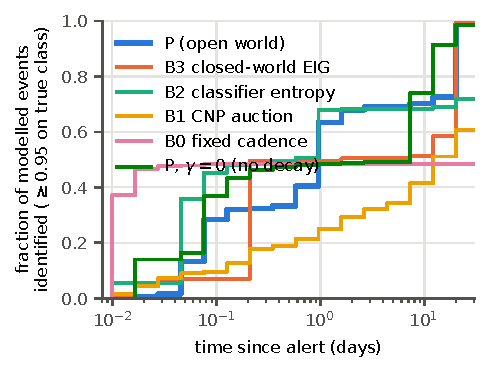
\includegraphics[width=\columnwidth]{generated/figures/fig1_tti.pdf}
\caption{H1. Cumulative fraction of modelled events whose posterior on the true class has reached 0.95, by time since alert (Nominal, test). B2 identifies the events it can identify earliest. P identifies almost all of them, but later. Closed-world EIG (B3) leaves many identifications to the final epochs.}
\label{fig:tti}
\end{figure}

\paragraph{H2, irreversibility: supported, with caveats.} Removing the decay term cut the information recovered about the true class's amplitude by \SimHtwoFast\ nats on fast classes and by \SimHtwoSlow\ on the slow GRB afterglow, a difference of \SimHtwoEst\ \SimHtwoCI. Kilonovae carry most of this effect (\SimDeltaKilonova), and shock cooling carries some of it (\SimDeltaShock). For the fastest class, the M-dwarf flare, the decay term actually lost information (\SimDeltaFlare; Fig.~\ref{fig:decay}). The effect also reversed under model error, because the wrong timescales mislead the urgency estimate (\SimHtwoModelErrorEst\ \SimHtwoModelErrorCI).

\begin{figure}[t]
\centering
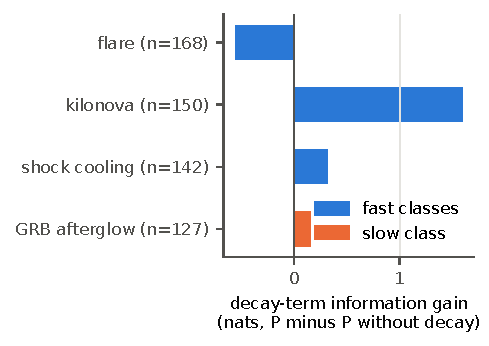
\includegraphics[width=\columnwidth]{generated/figures/fig2_decay.pdf}
\caption{H2. Information about the true amplitude gained from the decay term, per class (P minus P without it), Nominal test. The gain is positive for kilonova and shock cooling, near zero for the slow class, and negative for flares.}
\label{fig:decay}
\end{figure}

\paragraph{H3, open-world detection: supported.} At a 5\% false-alarm rate on modelled events, P's $P(h_0)$ detected \SimTprP\ of withheld events. A threshold on B3's closed-world posterior entropy detected \SimTprBthree\ (difference \SimHthreeEst\ points, 95\% CI \SimHthreeCI; Fig.~\ref{fig:rocsim}). The AUROC was \SimAucP\ for $P(h_0)$, against \SimAucBthree\ for B3 entropy and \SimAucBtwo\ for B2 entropy. Entropy computed on P's own measurements did no better (\SimAucPown), so the gain comes from the hypothesis itself and not from the measurements P chose. Without $h_0$, closed-world EIG was confidently wrong on \SimCwWhBthreeAll\ of withheld events, and P on \SimCwWhPAll. P made no false ``unknown'' calls on modelled events (\SimFaP) and kept the same modelled accuracy as B3 (\SimAccModPAll). H3 held in all three scenarios, but model error is the failure mode we predicted. Under model error, P called \SimFaPModelError\ of modelled events unknown, and its modelled accuracy fell to \SimAccModPModelError\ (B3: \SimAccModBthreeModelError).

\begin{figure}[t]
\centering
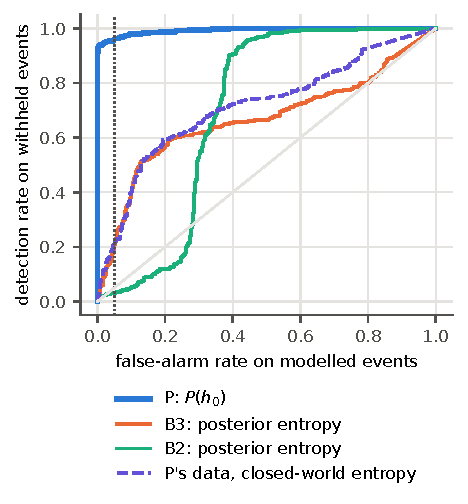
\includegraphics[width=\columnwidth]{generated/figures/fig3_roc_sim.pdf}
\caption{H3. ROC for separating withheld from modelled events (Nominal, test). The dotted line marks the preregistered 5\% false-alarm operating point.}
\label{fig:rocsim}
\end{figure}

\paragraph{Ablations.} Removing the adequacy term changed nothing we could measure. P$_{\beta=0}$ flagged \SimFlagNoAdeq\ of withheld events (P: \SimFlagP), with an AUROC of \SimAucAblNoAdeq\ (P: \SimAucAblP). Removing the decay term did matter. P$_{\gamma=0}$ took \SimObsAllNoDecay\ measurements instead of \SimObsAllP, flagged \SimFlagNoDecay, and was confidently wrong on \SimCwWhNoDecayAll\ of withheld events. So in this setting, the decay term helps open-world detection mainly by stopping the planner from spending its horizon too early, which leaves $h_0$ enough data to work with.

\begin{table*}[t]
\centering\scriptsize
\caption{Simulation test results (1000 events per scenario). Acc.\ mod.: accuracy on modelled events (\%). CW: confident-wrong rate (\%) on unmodelled (withheld) and modelled events. $\bar n_{\rm obs}$: measurements used, out of 5. Log score: mean log probability of the true outcome (closed-world strategies cannot express ``withheld'', so they are floored at $10^{-6}$).}
\label{tab:sim}
\begin{tabular}{llrrrrr}
\toprule
Scenario & Strategy & Acc.\ mod. & CW unmod. & CW mod. & $\bar n_{\rm obs}$ & log score \\
\midrule
Nominal & P (open world) & 100 & 6 & 0 & 4.2 & -0.19 \\
 & B3 closed-world EIG & 100 & 97 & 0 & 2.8 & -5.71 \\
 & B2 classifier entropy & 88 & 69 & 0 & 4.9 & -5.82 \\
 & B1 CNP auction & 80 & 75 & 0 & 3.2 & -5.92 \\
 & B0 fixed cadence & 79 & 1 & 0 & 5.0 & -5.92 \\
 & P, $\gamma=0$ (no decay) & 99 & 31 & 0 & 3.6 & -0.87 \\
 & P, $\beta=0$ (no adequacy) & 100 & 6 & 0 & 4.3 & -0.20 \\
\midrule
Crowding & P (open world) & 99 & 14 & 0 & 4.0 & -0.43 \\
 & B3 closed-world EIG & 100 & 94 & 0 & 3.0 & -5.82 \\
 & B2 classifier entropy & 94 & 80 & 0 & 4.8 & -5.88 \\
 & B1 CNP auction & 86 & 71 & 0 & 3.1 & -5.97 \\
 & B0 fixed cadence & 76 & 1 & 0 & 5.0 & -6.03 \\
 & P, $\gamma=0$ (no decay) & 100 & 31 & 0 & 3.4 & -0.96 \\
 & P, $\beta=0$ (no adequacy) & 99 & 14 & 0 & 4.1 & -0.43 \\
\midrule
Model error & P (open world) & 87 & 21 & 8 & 3.9 & -1.21 \\
 & B3 closed-world EIG & 99 & 96 & 1 & 2.9 & -6.11 \\
 & B2 classifier entropy & 81 & 29 & 4 & 5.0 & -6.32 \\
 & B1 CNP auction & 82 & 72 & 1 & 3.2 & -6.29 \\
 & B0 fixed cadence & 77 & 1 & 0 & 5.0 & -6.25 \\
 & P, $\gamma=0$ (no decay) & 93 & 26 & 6 & 3.4 & -1.32 \\
 & P, $\beta=0$ (no adequacy) & 86 & 21 & 8 & 3.9 & -1.21 \\
\bottomrule
\end{tabular}

\end{table*}



\section{Study 2: real ZTF replay}\label{sec:real}
\paragraph{Setup.} We replay spectroscopically classified ZTF Bright Transient Survey events \citep{Fremling2020,Perley2020} against the same satellites, propagated from element sets archived at each event's date. SN~Ia, II and Ibc are the modelled classes, with empirical $g$ and $r$ templates built only from events detected before 2020. Tidal disruption events, superluminous supernovae and SN~Ibn are the real unknowns. The truth at any epoch is a GP interpolation of the real light curve, so only the planner's measurements are simulated, and never beyond the last real detection.

\paragraph{Protocol.} A preregistered rule picked the configuration on the validation split: two bands, discrepancy $\kappa=0.5$ and a GP length scale of 5\,d. We fixed five hypotheses. H1 says P is less often confidently wrong than B3 on unmodelled events. H2 says $P(h_0)$ ranks unmodelled events above modelled ones (AUROC $>0.5$). On supernovae, H3 says P is not more than 5 points more often confidently wrong than B3, and H5 says it is not more than 5 points less accurate. H4 says colour raises the AUROC over a single-band arm on the same events. Each hypothesis has to pass on all three noise seeds (stratified paired bootstrap, $10^4$ resamples). The test events (\RealNEvents: \RealNModeled\ supernovae, \RealNWithheld\ unmodelled) had already been used twice, in the retrospective analyses, so this causal run is a declared third look.

\paragraph{Results.} Table~\ref{tab:real} shows both versions side by side. With causal measurements, H1--H4 pass and H5 fails. Closed-world EIG was confidently wrong on \RealCCwWhBthree\ of real unmodelled transients (\RealRCwWhBthree\ retrospectively), the auction baseline B1 on \RealCCwWhBone, and P on \RealCCwWhP. P labelled \RealCFlagP\ of unmodelled events as unknown, with an AUROC of \RealCAuc\ (Fig.~\ref{fig:rocreal}).

\begin{table*}[t]
\centering\scriptsize
\caption{Real ZTF replay, preregistered test results per noise seed: estimate [95\% CI]; $^\times$ marks a criterion not met on that seed. CW: confident-wrong rate. $\Delta$: P minus B3, or the colour arm minus the single-band arm for H4. The causal version (v3) is this paper's result. The retrospective version (v2) let planners measure earlier epochs after later ones and is shown only for comparison.}
\label{tab:real}
\begin{tabular}{lll@{\hspace{4pt}}l}
\toprule
& Seed & Causal (v3) & Retrospective (v2) \\
\midrule
H1 $\Delta$CW unmod. & 1 & -0.49 [-0.60, -0.36] & -0.60 [-0.72, -0.49] \\
 & 2 & -0.42 [-0.55, -0.30] & -0.67 [-0.77, -0.56] \\
 & 3 & -0.36 [-0.48, -0.25] & -0.60 [-0.73, -0.48] \\
\addlinespace
H2 AUROC $P(h_0)$ & 1 & +0.81 [+0.76, +0.86] & +0.80 [+0.75, +0.85] \\
 & 2 & +0.81 [+0.76, +0.86] & +0.80 [+0.75, +0.85] \\
 & 3 & +0.79 [+0.73, +0.84] & +0.77 [+0.71, +0.82] \\
\addlinespace
H3 $\Delta$CW mod. & 1 & -0.05 [-0.09, -0.01] & +0.00 [-0.06, +0.07]$^\times$ \\
 & 2 & -0.04 [-0.08, +0.00] & +0.04 [-0.03, +0.10]$^\times$ \\
 & 3 & -0.03 [-0.07, +0.01] & +0.06 [-0.01, +0.12]$^\times$ \\
\addlinespace
H4 $\Delta$AUROC colour & 1 & +0.19 [+0.13, +0.24] & +0.19 [+0.14, +0.24] \\
 & 2 & +0.18 [+0.12, +0.23] & +0.21 [+0.16, +0.27] \\
 & 3 & +0.24 [+0.18, +0.30] & +0.15 [+0.10, +0.20] \\
\addlinespace
H5 $\Delta$acc.\ mod. & 1 & +0.01 [-0.05, +0.07]$^\times$ & -0.08 [-0.14, -0.02]$^\times$ \\
 & 2 & +0.03 [-0.04, +0.09] & -0.06 [-0.13, +0.00]$^\times$ \\
 & 3 & -0.01 [-0.08, +0.05]$^\times$ & -0.08 [-0.14, -0.01]$^\times$ \\
\addlinespace
\bottomrule
\end{tabular}

\end{table*}

\begin{figure}[t]
\centering
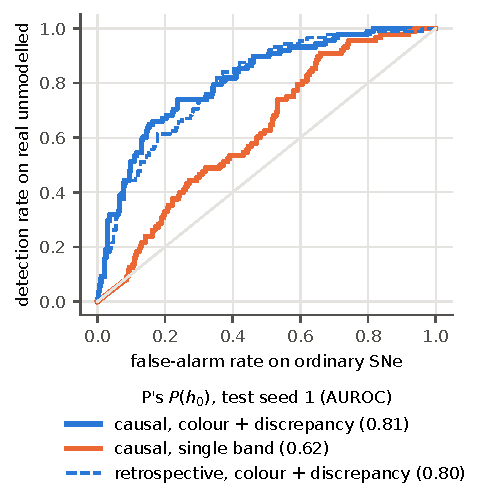
\includegraphics[width=\columnwidth]{generated/figures/fig4_roc_real.pdf}
\caption{Real data: ROC of the open-world planner's $P(h_0)$ for separating real unmodelled transients (TDE, SLSN, SN~Ibn) from ordinary supernovae, test seed 1. Colour plus model discrepancy is what makes $h_0$ usable, and enforcing causality leaves the curve almost unchanged.}
\label{fig:rocreal}
\end{figure}

\paragraph{What causality changed.} The retrospective runs failed H3 and H5. There, P paid for its safety on unknowns with more confident errors and lower accuracy on ordinary supernovae. With causality, H3 passes, the false-``unknown'' rate on supernovae falls from \RealRFaP\ to \RealCFaP, and P's supernova accuracy (\RealCAccModP) matches B3's (\RealCAccModBthree). H5 still fails, but narrowly. On two seeds, the lower confidence bound falls just below $-5$ points, so we cannot rule out a small loss. The cost moved to the unknowns instead: P now flags \RealCFlagP\ of them, against \RealRFlagP\ retrospectively. The reason is the measurement budget. With a time arrow, one-step utilities jump to a late, informative epoch and give up the earlier ones. P used \RealCObsP\ of its 5 measurements on average (B3 \RealCObsBthree, fixed-cadence B0 \RealCObsBzero), against \RealRObsP\ when it could go back in time. Fewer measurements make every posterior less confident, so confident errors drop on both populations, and some of P's detections go with them.



\section{A second decision rule: conformal open-set detection}\label{sec:conf}
The real-data replay left one hypothesis unmet. We could not show that the open-world planner is no less accurate on ordinary supernovae (H5). So we ran a second, independently preregistered study that goes after that cost directly, with two changes on top of the causal configuration of Section~\ref{sec:real}.

\paragraph{Method.} The first change is the conformal decision. After any planner's measurements $D$, we compute the prior-free score $s=\log p(D\mid h_0)-\max_c\log p(D\mid c)$ and flag ``unknown'' when $s>\tau$. Here $\tau$ is the largest, over known classes, of the split-conformal $(1-\alpha)$ quantile of $s$ on calibration events of that class. If the calibration events and new events of a class are exchangeable, the chance of a false ``unknown'' is at most $\alpha$ for every known class, for any planner and any mix of classes \citep{Vovk2005,Angelopoulos2023}. Otherwise, the closed-world decision stands. The second change is lookahead. Greedy one-step utilities end up with too few measurements, so a planner L adds $\lambda$ times the value of the best remaining later epochs to P's utility ($\lambda=0$ gives back P).

\paragraph{Protocol.} $\lambda=\ConfLambda$ was chosen on the validation split, and $\alpha=\ConfAlpha$ was fixed in advance. The calibration set and the sealed known-class test set were drawn fresh from Bright Transient Survey supernovae that no earlier analysis had used, split by a hash of the object name. That gave \ConfNCal\ calibration and \ConfNFresh\ sealed test supernovae, and the test ones were loaded for the first time in the test run. No unused unknown-class events were left, so the unknown-detection hypotheses (HC4--HC6) reuse the test split of Section~\ref{sec:real}, as an extra declared look. Each of the six hypotheses had to pass on all three noise seeds.

\begin{table*}[t]
\centering\scriptsize
\caption{Conformal open-set study, preregistered results per noise seed: estimate [95\% CI]; $^\times$ marks a criterion not met. Primary system: lookahead planner L with the conformal decision (C-L). $\Delta$: C-L minus closed-world EIG (B3), except HC6 (AUROC of $s$, L minus P). HC1 uses Clopper--Pearson intervals; HC2--HC4 and HC6 use the paired bootstrap.}
\label{tab:conf}
\begin{tabular}{llll}
\toprule
Hypothesis & Seed 1 & Seed 2 & Seed 3 \\
\midrule
HC1 false ``unknown'', sealed SNe ($\leq\alpha$) & +0.035 [+0.020, +0.055] & +0.061 [+0.042, +0.086] & +0.063 [+0.043, +0.089] \\
HC2 $\Delta$acc.\ SNe ($>-0.05$) & +0.082 [+0.039, +0.123] & +0.074 [+0.033, +0.115] & +0.059 [+0.012, +0.106] \\
HC3 $\Delta$CW SNe ($<+0.05$) & -0.027 [-0.057, +0.002] & -0.049 [-0.078, -0.020] & -0.012 [-0.043, +0.018] \\
HC4 $\Delta$CW unknowns ($<0$) & -0.239 [-0.375, -0.102] & -0.261 [-0.409, -0.114] & -0.193 [-0.341, -0.045] \\
HC5 unknowns flagged ($>\alpha$) & +0.420 [+0.316, +0.530] & +0.545 [+0.436, +0.652] & +0.432 [+0.327, +0.542] \\
HC6 $\Delta$AUROC, L$-$P ($>0$) & +0.012 [-0.013, +0.038]$^\times$ & +0.031 [+0.006, +0.058] & +0.039 [+0.005, +0.075] \\
\bottomrule
\end{tabular}

\end{table*}

\paragraph{Results.} Five of the six hypotheses passed (Table~\ref{tab:conf}). On the sealed supernovae, the false-``unknown'' rate was \ConfFa, inside the certified \ConfAlphaPct\ (HC1 \ConfHCOneVerdict). C-L was \ConfAccGain\ more accurate than closed-world EIG (HC2 \ConfHCTwoVerdict, the re-test of H5), with no more confident errors (HC3 \ConfHCThreeVerdict). On the real unknowns, C-L flagged \ConfFlag\ (HC5 \ConfHCFiveVerdict) and was less often confidently wrong than B3 (HC4 \ConfHCFourVerdict). Lookahead did not reliably improve how unknowns are ranked compared with P (HC6 \ConfHCSixVerdict; AUROC difference \ConfAucGain, not significant on seed 1).

\paragraph{Where the gains come from, and what they cost.} With causal measurements, P without the conformal layer was already as accurate as B3 on the sealed supernovae (\ConfAccFreshP\ against \ConfAccFreshBthree), with a raw false-``unknown'' rate of \ConfRawFaFreshP. So much of the earlier H5 failure came from the retrospective protocol. Lookahead added accuracy (\ConfAccFreshCL) by using more of the budget (\ConfObsL\ measurements against \ConfObsP\ for P). The conformal layer works with any planner. Applied to closed-world EIG, it flagged \ConfFlagBthreeConf\ of unknowns while keeping B3's supernova accuracy close to its own (\ConfAccFreshBthreeConf). The cost shows up on the unknowns. C-L was confidently wrong on \ConfCwUnkCL\ of them, against \ConfCwUnkP\ for P's Bayesian decision and \ConfCwUnkBthree\ for B3. The two rules buy different things. The conformal rule buys a certified false-alarm rate and accuracy on known classes. The Bayesian $h_0$ buys fewer confident errors on unknowns, but with no guarantee. Which one to deploy depends on which error costs more.



\paragraph{A guarantee with no calibration, on real events.} The conformal rule needs calibration events, so we also tested the e-process of Eq.~\eqref{eq:eprocess} on the same real data, with no tuning at all. We replayed every planner draw for draw, so each one took exactly the measurements reported above, and then raised ``unknown'' the first time $E_t$ reached $1/\alpha=10$. Real light curves never match a template exactly, so the null hypothesis is only roughly true here, and that is what we wanted to test. On the \EFreshN\ sealed supernovae, P's false-``unknown'' rate was \EFreshFa\ over three noise seeds, with an upper bound of \EFreshFaUpper\ against the promised 10\% (HR1 \EHROneVerdict). On the \EWithheldN\ real unknowns it flagged \EDet, with a lower bound of \EDetLower\ (HR2 \EHRTwoVerdict). This is less than the \RealCFlagP\ that $P(h_0)$ flagged on the same events, but it comes with a guarantee that holds at every step. The e-process also works on any planner. On the closed-world planner's measurements it flagged \EDetBthree\ of the unknowns, and on the lookahead planner's \EDetL, because those planners take more measurements per event. Their false-``unknown'' rate stayed low as well (\EFreshFaBthree\ for the closed-world planner). So a planner that ignores $h_0$ can still be given a safe ``unknown'' label afterwards, just by adding this test on top.

\section{Study 4: a fleet that cannot always talk}\label{sec:fleet}

\paragraph{Setup.} Each episode has four transients alerted together, drawn as in Study~1, and eight real-orbit satellites. Each satellite can take one measurement per epoch and three in total. We compare four strategies. O has ideal links and runs one fleet-wide auction. A$_R$ runs an auction inside each linked group, for link ranges $R\in\{1,2,3,5\}\times10^3$\,km. K$_R$ shares knowledge the same way, but each spacecraft plans alone. G has no links at all. P's utility is frozen from Study~1. We chose reserve prices on validation episodes with a rule declared beforehand (O: \FleetReserveO, G: \FleetReserveG, A: \FleetReserveA, K: \FleetReserveK), and A and K landed at the edge of the grid. The preregistered test used \FleetNEpisodes\ episodes (\FleetNEvents\ events, \FleetNModeled\ of them modelled). Links are scarce, so a satellite pair is linked only \FleetLinkUpOne\ of the time at 1000\,km and \FleetLinkUpFive\ at 5000\,km.

\paragraph{Results.} Ideal communication raised accuracy on modelled events by \FleetHFourOneEst\ points over isolated spacecraft (\FleetHFourOneCI; H4.1 \FleetHFourOneVerdict). Realistic links did not measurably help. A$_{5000}$ minus G was \FleetHFourTwoEst\ points (\FleetHFourTwoCI; H4.2 \FleetHFourTwoVerdict), so ideal links beat realistic ones by \FleetHFourThreeEst\ points (\FleetHFourThreeCI; H4.3 \FleetHFourThreeVerdict). Coordinating plans added nothing on top of sharing knowledge. A$_{5000}$ minus K$_{5000}$ was \FleetHFourFourEst\ points (\FleetHFourFourCI), inside the preregistered $\pm5$ (H4.4 \FleetHFourFourVerdict). The e-process made at most \FleetHEOneMaxK\ false ``unknown'' call in \FleetHEOneN\ modelled events, for every strategy (HE1 \FleetHEOneVerdict). When spacecraft averaged the last e-values they had heard, they raised \FleetHETwoK\ false alarms in \FleetHETwoN\ (event, spacecraft) pairs (HE2 \FleetHETwoVerdict). The e-process paid for this safety in power, so under O it detected \FleetEDetO\ of the unknowns, where $P(h_0)$ flagged \FleetFlagO.

\begin{table}[t]
\centering\footnotesize
\caption{Fleet test results (nominal, preregistered reserves). Acc.\ mod.: accuracy on modelled events (\%); CW unk.: confidently wrong on unknowns (\%); Flag unk.: unknowns labelled $h_0$ (\%); $\bar n_{\rm obs}$: measurements per event; Stale: share of already-taken records a spacecraft does not yet know (\%).}
\label{tab:fleet}
\begin{tabular}{lrrrrrrr}
\toprule
Strategy & Acc.\ mod. & CW unk. & Flag unk. & AUROC & log score & $\bar n_{\rm obs}$ & Stale \\
\midrule
Ideal links (oracle) & 87 & 8 & 48 & 0.93 & -0.80 & 5.1 & 0 \\
Auction, ISL $\leq$5000\,km & 75 & 0 & 45 & 0.90 & -0.88 & 3.7 & 29 \\
Knowledge only, ISL $\leq$5000\,km & 74 & 0 & 42 & 0.89 & -0.91 & 3.8 & 29 \\
Auction, ISL $\leq$1000\,km & 72 & 1 & 39 & 0.88 & -0.95 & 3.8 & 45 \\
No links & 76 & 4 & 39 & 0.88 & -0.99 & 5.4 & 88 \\
\bottomrule
\end{tabular}

\end{table}

\begin{figure}[t]
\centering
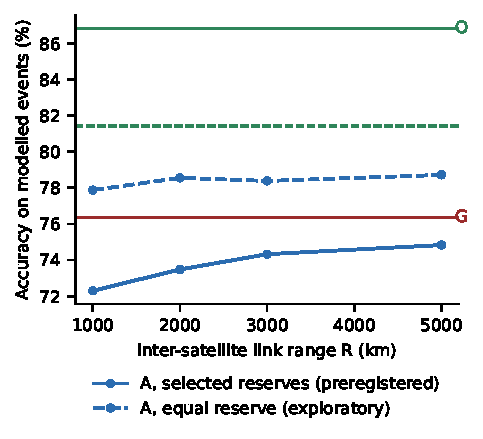
\includegraphics[width=0.62\textwidth]{generated/figures/fig5_fleet.pdf}
\caption{Accuracy against inter-satellite link range. Horizontal lines: ideal links (O, green) and none (G, red). Solid: preregistered reserves. Dashed: all strategies at one reserve (exploratory, added after the test).}
\label{fig:fleet}
\end{figure}

\paragraph{Why H4.2 failed.} Our selection rule maximised log score, and it picked a higher reserve for A than for G, so A took \FleetObsA\ measurements per event against \FleetObsG. A was better calibrated (log score \FleetLsA\ against \FleetLsG, and confidently wrong on \FleetCwUA\ of unknowns against \FleetCwUG), but it was not more accurate. We were not satisfied with a result that mixed two effects, so we added an exploratory run with every strategy at the same reserve. Realistic links then gave \FleetExAminusGEst\ points (\FleetExAminusGCI) and ideal links gave \FleetExOminusGEst\ (\FleetExOminusGCI), while coordination still added nothing (\FleetExAminusKEst, \FleetExAminusKCI). The same oracle reached \FleetAccO\ with its own reserve and \FleetExAccO\ with the common one. So the choice of when to spend a measurement moved accuracy about as much as perfect communication did.

\paragraph{A second preregistered test.} An exploratory look is not evidence, so we wrote five new hypotheses and tested them on a fresh seed (\FleetBNEvents\ events). All three runs share identical events, so every comparison is paired. With equal spending, realistic links now helped, and A$_{5000}$ minus G was \FleetBOneEst\ points (\FleetBOneCI; B1 \FleetBOneVerdict). Coordination again added nothing (\FleetBTwoEst, \FleetBTwoCI; B2 \FleetBTwoVerdict). The spending rule alone moved the oracle by \FleetBThreeEst\ points (\FleetBThreeCI; B3 \FleetBThreeVerdict).

\paragraph{Where the satellites sit.} We also tested a fleet of eight satellites drawn from one orbital plane. It is far better connected, with links up \FleetDenseLinkUpOne--\FleetDenseLinkUpFive\ of the time against \FleetLinkUpOne--\FleetLinkUpFive\ for the spread fleet. Even with ideal links, it was \FleetBFourEst\ points less accurate (\FleetBAccODense\ against \FleetBAccOSparse, \FleetBFourCI; B4 \FleetBFourVerdict). Satellites that share a plane lose and regain sight of a target together, so the fleet measures each event at fewer distinct epochs (\FleetBFiveEst\ epochs per event, \FleetBFiveCI; B5 \FleetBFiveVerdict). For a follow-up fleet, the spread of the satellites over the sky matters more than how well they can talk.

\paragraph{Under model error.} When every template's timescale is off by 30\%, the e-process's false-``unknown'' rate rises to \FleetMEFalseUnknownO\ for O and \FleetMEFalseUnknownG\ for G. The hypothesis the e-process tests, that the data come from the templates, is now false, so these alarms are the guarantee working as stated. The fleet with the most data noticed this most often, which is what a working test should do.

\section{Discussion}\label{sec:disc}

\paragraph{The belief does the work.} The one finding that holds in every study is that keeping $h_0$ in the posterior stops confident misclassification of the unknown. The utility term built to test $h_0$ ($\beta$) made no measurable difference. In simulation, a closed-world entropy threshold on P's own measurements reached an AUROC of only \SimAucPown, against \SimAucP\ for $P(h_0)$ on the same measurements. So what makes the unknown recognisable is a hypothesis space that can name it, plus colour on real data. This goes against the intuition that a planner must hunt for anomalies. It first needs to be able to say ``none of these''.

\paragraph{Two kinds of guarantee.} The Bayesian $h_0$ made the fewest confident errors on real unknowns, but it promises nothing about false alarms. The conformal threshold gets a certified false-alarm rate from exchangeable calibration events, and that rate holds at the end of the budget. The e-process gets validity at every step and on any planner from the model itself, and we can average it across spacecraft whose data overlap. It pays in power, and in principle it is only as good as the templates, but on real supernovae that never match a template exactly it still stayed at \EFreshFa\ false alarms. So the choice depends on which error costs more, and on whether we trust the calibration set or the physics more.

\paragraph{The time arrow.} An earlier version of our pipeline let planners measure earlier epochs after later ones. This did not bias the comparison between strategies, but it changed the conclusions. Once measurements were causal, adaptive planners used about half of their budget, posteriors became less confident, and the supernova-cost hypothesis of Study~2 went from fail to pass. That is why we think benchmarks for follow-up planning should check the time order of every chosen sequence.

\paragraph{What a fleet needs.} Three things moved accuracy, and their order surprised us. Where the satellites are mattered most, since a spread fleet beat a single plane by \FleetBFourEst\ points. When they spend a measurement came next (\FleetBThreeEst). Whether they share what they have seen came last (\FleetBOneEst\ for realistic links and \FleetHFourOneEst\ for ideal ones). Coordinating plans added nothing in either test once knowledge was shared. So for small science fleets, we would invest in orbital diversity and in getting observations to each other, before negotiating who observes. CRDT sharing kept this safe, and no record was ever counted twice, whatever path it took.

\paragraph{What did not work.} The planner was not the fastest identifier. A cheap disagreement heuristic identified the events it could identify sooner, so H1 failed. The decay term helped kilonovae, but it reversed for flares and under model error. Realistic crosslinks failed their first preregistered test (H4.2). The selected spending rules differed between strategies, so we tested again with equal spending, and then they passed (B1). The real-data replay could not show supernova accuracy within five points of the closed-world planner (H5) until the conformal and lookahead study.

\paragraph{Limitations.} Simulated light curves are analytic shapes, and amplitude is their only parameter. The decay term is a squared signal-to-noise proxy. There is no slew, exposure or link-budget model, and fleet links are purely geometric. On real data, we resample measurements from interpolated light curves and assume two-band imaging, and the test events were examined more than once, which we declared in advance. In the fleet study, two reserve prices sit at the edge of the validation grid, the satellites use old element sets, and the equal-reserve run in Study~4 is an extra look at the first test seed.

\section{Conclusion}\label{sec:concl}
For autonomous follow-up of fading transients, give the planner a way to say ``none of the above''. In simulation and on real ZTF events, this is the part of the method that keeps stopping confident misclassification of the unknown, and once measurements are causal it costs little on ordinary events. If a guaranteed false-alarm rate matters, a conformal threshold gives one at the end of the budget, and an e-process gives one at every step and across spacecraft without calibration data. A one-step utility does not manage urgency well, so we would not rely on it for that, and every follow-up study should check the time arrow. For a fleet, spread the satellites out, decide carefully when to spend, and share what you have seen before negotiating what to see next.

\backmatter

\bmhead{Acknowledgements}
This work was carried out under the guidance of Dr.~Smitha Shekar B and Dr.~Harish G, Department of Computer Science and Engineering, Dr.\ Ambedkar Institute of Technology, Bengaluru.

\section*{Declarations}

\begin{itemize}
\item Funding: Not applicable. This research received no external funding.
\item Competing interests: None.
\item Data availability: ZTF Bright Transient Survey light curves are public. Every per-event result, preregistration file and the scripts that generate every number, table and figure in this paper are in the code repository below.
\item Code availability: \url{https://github.com/joycemalik/orbitalnet-dashboard}, branch \texttt{research/open-world-planner}.
\item Author contributions: All authors (J.M., A.H., M.B. and S.S.) contributed to the conception and design of the framework and to the writing of the manuscript. All authors read and approved the final manuscript.
\end{itemize}

\bibliographystyle{mnras}
\bibliography{refs}

\end{document}
